\documentclass{erauthesis}
\department{Mechanical Engineering}
\chair{Eric Coyle, Ph.D}
\dean{James Gregory, Ph.D.}
\dgc{Lon Moeller, J.D.}
\depchair{Patrick Currier, Ph.D.}
\advisortitle{Committee chair}
\usepackage{graphicx}
\usepackage{amsmath}
\usepackage{amssymb}
\usepackage{textcomp, gensymb}
\usepackage{array}
\usepackage{enumitem}
\usepackage{xcolor}
\usepackage{algorithm}
\usepackage{algpseudocode}

\usepackage{subcaption} % for multiple image figures
% \usepackage[style=authoryear]{biblatex} % or numeric, apa, etc.
% \addbibresource{Dissertation.bib}         % your Zotero export

% pkgs for .mermaid chart
\usepackage{tikz}
\usetikzlibrary{shapes.geometric, arrows}

% acronyms
\usepackage[nolist]{acronym} 

% preamble for Lit-review tables:
\usepackage{tabularx,ragged2e,makecell}
\renewcommand\theadfont{\bfseries}
\renewcommand\cellalign{tl} % top-left for makecell
\newcolumntype{L}[1]{>{\RaggedRight\arraybackslash}p{#1}}
\newcolumntype{Y}{>{\RaggedRight\arraybackslash}X}

\title{A STUDY IN OBJECT DETECTION AND CLASSIFICATION
PERFORMANCE BY SENSING MODALITY FOR AUTONOMOUS
SURFACE VESSELS} % the title should be included here
\author{Daniel P. Lane} 
\graduation{December}{2025}
\advisor {Eric Coyle} %Committe chair


\coadvisor{Subhradeep Roy} % If you do not have a co-advisor, delete this whole command

\committememzero{Xxxx X. Xxxxxxxxx, Ph.D.} % If you have a co-advisor, do not edit this member name
%% Enter the name of the committee members
\committememone{Patrick Currier}
\committememtwo{Monica Garcia}
\committememthree{Jianhua Liu}
\committememfour{TBD}



%\signaturepush{-2.0}									

\usepackage{subfiles} % Best loaded last in the preamble

\begin{document}


\frontmatter

\maketitle

% \makesignature
\makeatletter 
\advance\fau@frontstage by 1  % Skip signature page but maintain counter
% \makeanother
\begin{acronym}[GB-CACHE] % Give the longest label here so that the list is nicely aligned
\acro{ASV}{Autonomous Surface Vessel}
\acro{USV}{Unmanned Surface Vessel}
\acro{ERAU}{Embry-Riddle Aeronautical University}
\acro{GB-CACHE}{Grid-Based Clustering and Concave Hull Extraction}
\acro{GPS}{Global Positioning System}
\acro{WAM-V}{wave-adaptive modular vessel}
\acro{HDR}{High Dynamic Range}
\acro{IMU}{Inertial Measurement Unit}
\acro{INS}{Inertial Navigation System}
\acro{IoU}{Intersection over Union}
\acro{LiDAR}{Light Detection and Ranging}
\acro{mAP}{mean Average Precision}
\acro{MPC}{model predictive control}
\acro{RGB}{Red, Green, Blue}
\acro{ROI}{Region of Interest}
\acro{ROS}{Robot Operating System}
\acro{USV}{Unmanned Surface Vessel}
\acro{YOLO}{You Only Look Once}
\acro{YOLOv8}{You Only Look Once ver. 8.0}
\acro{LWIR}{Long-Wave Infrared}
\acro{FPS}{Frames per Second}
\acro{EFL}{effective focal length}
\acro{FOV}{Field of View}
\acro{LAN}{Local Area Network}
\acro{SEI}{Supplemental Enhancement Information}
\acro{NAL}{Network Abstraction Layer}
\acro{NTP}{Network Time Protocol}
\acro{PTP}{Precision Time Protocol}
\acro{RTP}{Real-time Transport Protocol}
\acro{RTSP}{Real-time Streaming Protocol}
\acro{UDP}{User Datagram Protocol}

\end{acronym}

\begin{acknowledgements}
% \raggedright
I would like to express my deepest gratitude to my friends, family, and especially my parents, whose unwavering love, encouragement, and support have sustained me throughout my academic journey. Their belief in me has been a constant source of strength and motivation.

I am sincerely thankful to my advisor, Dr. Coyle, for his mentorship and steady guidance throughout this research. He has taught me lessons both in and beyond the classroom that will stay with me for a lifetime, and for that, I will be forever grateful.

I would also like to extend a special thanks to my co-advisor, Dr. Roy, who first introduced me to the world of academic research rigor. His guidance shaped the foundation of my development as a researcher and helped me grow into the kind of professional and scholar I aspired to become.

Finally, I wish to acknowledge the faculty and staff of the Department of Mechanical Engineering for their continued support of my academic and professional growth. 
Their commitment to excellence in teaching and research has profoundly influenced my development as both a student and an educator.

\vspace{3mm}

This work was supported in part by NEEC grant N00174-22-1-0012 through NUWC Keyport.
Any opinions, findings, conclusions, or recommendations expressed in this material are those of the authors and do not necessarily reflect the views of the Department of the Navy or Office of Naval Research.
\end{acknowledgements}

\begin{abstract}
	% \raggedright Researcher: Daniel P. Lane
 % \\Title: A study in object detection and classification performance by sensing modality for autonomous surface vessels \\Institution:	Embry-Riddle Aeronautical University\\Degree:	Doctor of Philosophy in Mechanical Engineering\\Year:	2025 \\
 This research addresses the critical gap in quantitative performance comparison between \ac{LiDAR} and vision-based sensing for real-time maritime object detection on autonomous surface vessels.
 Using \ac{ERAU}'s Minion platform and 2024 Maritime RobotX Challenge data, this study evaluates \ac{GB-CACHE} \ac{LiDAR} processing against \ac{YOLO} vision detection across six maritime object categories. The methodology encompasses real-time performance analysis, multi-sensor calibration, and sensor fusion for bounding box confidence integration.
 Performance metrics include precision, recall, \ac{mAP}, training requirements, and computational efficiency. 
 % Results demonstrate [key performance finding] and establish [fusion outcome]. 
 The research provides quantitative baselines for maritime sensing modality selection and validated calibration procedures enabling improved autonomous navigation in complex maritime environments.
 
 % Lorem ipsum dolor sit amet... This is a summative abstract, not just a list of topics.  Include relevant information including conclusions and recommendations.  Limit to 150 words; spell out abbreviations; citations not needed.

\end{abstract}
\pagetableofcontents
\clearpage
\listoftables					% Or \nolistoftables if there are no 
\clearpage
\listoffigures					% Or \nolistoffigures if there are no 




\mainmatter
\newpage
\chapter{Introduction}


The rise of autonomous systems is transforming various industries, and the maritime sector is no exception. Autonomous surface vessels (ASVs) have the potential to improve safety in traditionally human-operated vessels, taking on dull, dirty, and dangerous jobs.
A critical component of these systems is the ability to accurately perceive the surrounding environment. 
Real-time object detection and classification are essential for autonomous navigation and situational awareness, ensuring safe and efficient operation in maritime environments. 
While the automotive industry has seen significant advances in autonomous vehicle technology, these have yet to be fully realized for marine ASVs.
This translates directly into the volume of literature published on automotive and marine object detection strategies. 
While detection strategies can be adapted from the automotive environment, the marine environment is less structured yet retains significant complexity and object density, particularly in littoral zones.
Maritime object detection is challenging due to turbulent waves, sea fog, water reflection, and fluctuating lighting conditions. 
For close to mid-range detection, typical marine radar sensors provide poor fidelity.
Cameras and LiDAR provide much denser information but can still struggle in inclement weather or poor lighting conditions. 
These limitations highlight the need for more robust systems and highlight where combining the data from multiple sensors through data fusion can provide significant performance benefits. 
However, more research is required to find optimal real-time fusion strategies for maritime applications.
This study investigates the comparative performance of LIDAR and camera-based object detection and classification systems in well-lit maritime environments with near-optimal weather conditions. 
It examines sensor fusion strategies, training efficiency, and performance metrics on a range of common maritime objects, including navigational markers and small to medium-sized vessels, and aims to find an efficient real-time fusion strategy that leverages the best performance of each sensor.

% The novel contributions of this paper may be broken down as:
% \begin{itemize}
%     \item 
% \end{itemize}

% \section{Introduction} \label{introduction}

\section{Significance of Study} \label{significance_of_study}
\subfile{sections/significance_of_study}

\section{Problem Statement: Performance Comparison Gap} \label{problem_statement1}
\subfile{sections/problem_statement1}

\chapter{Literature Review} \label{litReview}



%%%%%%%%%%% %%%%%%%%%%% %%%%%%%%%%% %%%%%%%%%%%
% \section{Autonomous Surface Vessel Perception}

% Autonomous surface vessels (\acp{USV}) have evolved into critical platforms capable of performing operations that are too dangerous, repetitive, or time-consuming for humans. They support missions such as oceanographic mapping, search and rescue, port surveillance, and environmental monitoring \cite{liebergall, eckstein2024}. Their autonomy depends on robust sensing, reliable perception, and adaptive decision-making systems that can function under dynamic maritime conditions \cite{bai2022}.
% As autonomy levels increase from remote operation to full autonomy, so do the complexity and reliability requirements for perception systems \cite{zotero-item-1911,huang}.
% This motivates the development of sensor fusion approaches that can maintain performance despite environmental challenges and sensor degradation.

% % % ---

% \section{Sensing Modalities for Environmental Perception}

% Autonomous systems rely on multimodal sensing to perceive their surroundings. Among these, cameras and LiDAR are the most common combination, providing complementary information: cameras offer rich semantic and color cues, while LiDAR provides accurate three-dimensional spatial structure independent of illumination \cite{yeong2021}. 
% Additional modalities such as radar, sonar, GPS/INS, and thermal/infrared imaging extend perception capabilities under specific conditions.
% Table~\ref{table:sensor_modalities} summarizes the characteristics of common maritime sensing modalities. 

% \begin{table}[htbp]
% \centering
% \caption{Comparison of sensing modalities for maritime perception applications.}
% \label{table:sensor_modalities}
% \small
% \renewcommand{\arraystretch}{1.2}
% \begin{tabularx}{\textwidth}{L{1.8cm} L{3.4cm} L{3.4cm} Y}
% \hline
% \thead{Sensor} & \thead{Strengths} & \thead{Weaknesses} & \thead{Maritime Challenges} \\
% \hline\hline
% \textbf{Thermal / IR} & 
% Low-light capability; temperature contrast detection & 
% Lower resolution; atmospheric absorption; limited range & 
% Reduced contrast over water, fog attenuation \\
% \textbf{Camera (RGB)} & 
% High resolution; semantic/texture cues; mature deep learning models & 
% Lighting dependent; no direct depth; limited range in haze & 
% Glare, horizon dominance, low texture, HDR requirements \\
% \textbf{LiDAR} & 
% Accurate 3D geometry; illumination independent; precise range & 
% Sparse returns; limited semantics; atmospheric attenuation & 
% Water reflections, spray interference, platform motion \\
% \textbf{Radar} & 
% Long range; weather penetration; detect metallic objects well & 
% Low resolution; limited object classification; clutter & 
% Sea clutter, false returns from waves, multipath \\
% \textbf{Sonar} & 
% Subsurface detection; debris/obstacle mapping & 
% Underwater only; slow update rate; narrow FOV & 
% Turbidity, biological noise, platform motion \\
% \hline
% \end{tabularx}
% \end{table}

% \textbf{Synthesis:} 
% % No single sensor modality addresses all maritime perception challenges. 
% For this research, the complementary nature of high-resolution RGB cameras and precise 3D LiDAR provides a balanced foundation for exploring multimodal fusion under representative maritime conditions.
% Cameras provide semantic richness but fail under extreme lighting; LiDAR offers geometric precision but struggles with reflective surfaces; radar penetrates weather but lacks resolution. 
% This inherent complementarity motivates multimodal fusion approaches that leverage each sensor's strengths while compensating for individual weaknesses. 
% The maritime environment's dynamic lighting, reflective surfaces, and atmospheric variability make sensor fusion not merely beneficial but essential for reliable autonomous operation.

% % % ---

% \section{Object Detection with Visual and LiDAR Data}

% \subsection{Vision-Based Object Detection}

% Deep learning–based object detection has become the standard for visual perception. Architectures such as Faster R-CNN, SSD, and YOLO families have demonstrated real-time performance on embedded hardware \cite{he2016, ultralytics}. These models extract hierarchical features through convolutional layers to locate and classify objects in 2D images.

% Modern vision-based detection methods rely heavily on transfer learning from large-scale datasets such as COCO (Common Objects in Context) and ImageNet. Pre-trained feature extractors learn generalizable representations from millions of annotated images, enabling rapid adaptation to new domains with limited data. However, this paradigm introduces domain adaptation challenges when applied to maritime environments. Maritime scenes differ fundamentally from terrestrial datasets: they exhibit low texture diversity (dominated by sky and water), extreme dynamic range (from shadowed objects to sun glare), horizon-dominated compositions that violate typical object placement assumptions, and specular reflections that obscure object boundaries. These characteristics reduce the effectiveness of features learned from terrestrial images, often requiring domain-specific fine-tuning or maritime-specific training datasets to recover acceptable performance.

% Recent single-stage detectors prioritize inference speed, making them suitable for embedded deployment. YOLOv5 through YOLOv8 \cite{ultralytics} achieve real-time frame rates on GPU-accelerated platforms while maintaining competitive accuracy through architectural innovations such as CSPNet backbones, PANet feature fusion, and anchor-free detection heads. EfficientDet \cite{tan2020} employs compound scaling to balance model depth, width, and input resolution, achieving state-of-the-art accuracy-efficiency trade-offs. While EfficientDet achieves strong performance in terrestrial datasets, its reliance on dense texture cues limits performance under maritime HDR conditions where large image regions contain minimal semantic information.

% \textbf{Maritime-Specific Challenges:} The marine environment introduces unique failure modes for vision-based detection. Sun glare creates saturated image regions that eliminate feature information. Water reflections produce mirror-image artifacts that can be misclassified as objects. Low-texture backgrounds provide insufficient gradient information for feature extraction. Horizon lines create strong edges that can interfere with object localization. High dynamic range (HDR) scenes—where bright sky coexists with shadowed vessels—exceed the capture range of standard cameras, forcing a trade-off between overexposed highlights and underexposed shadows. These challenges motivate the investigation of HDR imaging and sensor fusion to maintain detection performance under adverse maritime conditions.

% \subsection{LiDAR-Based Object Detection}

% LiDAR-based detection networks process 3D point clouds to identify objects by geometry and reflectivity. Approaches are categorized as:
% \begin{itemize}
%     \item \textbf{Point-based:} directly operate on raw points (e.g., PointNet, PointNet++ \cite{garcia-garcia2016}), learning permutation-invariant features through symmetric functions and local neighborhood aggregation;
%     \item \textbf{Voxel-based:} use 3D convolutions on discretized volumes (e.g., VoxelNet \cite{zhou2018a}), enabling efficient spatial reasoning at the cost of discretization artifacts;
%     \item \textbf{Hybrid:} fuse voxel and point features (e.g., PV-RCNN \cite{shi2021}), combining the efficiency of voxel representations with the precision of point-based refinement.
% \end{itemize}

% The automotive industry has driven significant advances in LiDAR-based detection, with models trained on large-scale datasets such as KITTI, Waymo Open Dataset, and nuScenes. However, automotive-trained models face substantial performance degradation in maritime environments due to fundamental differences in point cloud characteristics. Water surfaces produce sparse, noisy returns rather than the dense ground-plane structure assumed by automotive models. LiDAR beams undergo specular reflection from calm water, resulting in few or no returns, while choppy water creates scattered, inconsistent reflections. Maritime objects (vessels, buoys, navigation markers) exhibit geometries and reflectance properties distinct from vehicles and pedestrians. Atmospheric conditions such as fog, rain, and spray attenuate LiDAR signals and introduce measurement noise. These factors necessitate maritime-specific training data and potentially modified network architectures to achieve reliable object detection.

% Recent developments in transformer-based architectures and bird's-eye-view (BEV) representations offer promising directions for maritime LiDAR detection. BEVFusion \cite{liu2023bevfusion} unifies camera and LiDAR features in a shared BEV space, enabling efficient spatial alignment without explicit geometric projection. TransFusion \cite{bai2022transfusion} employs transformer attention mechanisms to aggregate multi-scale features across modalities. Point Transformer \cite{zhao2021} applies self-attention directly to point clouds, capturing long-range dependencies that may help distinguish maritime objects from complex water-surface backgrounds. However, these architectures remain largely unvalidated in maritime contexts, and their computational requirements may exceed embedded platform constraints.

% \textbf{Comparative Challenges for LiDAR vs. Vision:} LiDAR and camera-based detection face orthogonal failure modes in maritime environments. Vision systems fail under extreme lighting (glare, low-light) but excel when texture and semantic cues are available. LiDAR maintains functionality across lighting conditions but degrades under specular reflections and atmospheric interference. Vision detects low-reflectance objects (dark vessels, rubber inflatables) that may produce weak LiDAR returns, while LiDAR reliably measures geometry even when visual appearance is ambiguous. This complementarity suggests that fusion approaches combining both modalities can achieve more robust detection than either sensor alone—motivating the investigation of late-fusion strategies that preserve each modality's independent strengths while combining their outputs.

% % ---

% \section{Sensor Fusion Paradigms}

% Sensor fusion combines multiple sensing modalities to overcome individual weaknesses and increase robustness. Fusion strategies are typically categorized as:
% \begin{itemize}
%     \item \textbf{Early Fusion (Data-level):} combine raw sensor data before feature extraction, e.g., projecting LiDAR points into the image frame.
%     \item \textbf{Mid Fusion (Feature-level):} merge intermediate features extracted separately from each modality.
%     \item \textbf{Late Fusion (Decision-level):} integrate independent detections using spatial, probabilistic, or learned weighting.
% \end{itemize}

% Table~\ref{table:fusion_paradigms} summarizes the characteristics, advantages, and representative examples of each fusion paradigm.

% \begin{table}[htbp]
% \centering
% \caption{Comparison of sensor fusion paradigms for multimodal perception.}
% \label{table:fusion_paradigms}
% \small
% \setlength{\tabcolsep}{4pt}
% \renewcommand{\arraystretch}{1.15}
% \begin{tabularx}{\textwidth}{L{3.0cm} Y Y}
% \hline
% \thead{Fusion Level} & \thead{Description and Mechanism} & \thead{Advantages / Disadvantages \& Examples} \\
% \hline\hline

% \textbf{Early (Data level)} &
% Merge raw data before features (e.g., project LiDAR to image; depth alignment). &
% \textit{+} Joint feature learning; geometric context. 
% \ \textit{–} Needs precise calibration/sync; sensitive to noise. 
% \ \textit{Ex:} PointPainting, MV3D. \\

% \textbf{Mid (Feature level)} &
% Fuse intermediate features (image/BEV/3D feature maps; cross-modal layers). &
% \textit{+} Balance of robustness and shared learning. 
% \ \textit{–} Feature alignment is complex; higher compute. 
% \ \textit{Ex:} AVOD, DeepFusion, BEVFusion. \\

% \textbf{Late (Decision level)} &
% Fuse independent detections (probabilistic weighting, rules, ensembles). &
% \textit{+} Modular; efficient; resilient to missing sensors. 
% \ \textit{–} Limited joint context learning; relies on detector quality. 
% \ \textit{Ex:} Ensemble CNNs; probabilistic fusion. \\
% \hline
% \end{tabularx}
% \end{table}

% \textbf{Early Fusion (Data-level):} Early fusion methods combine raw sensor inputs before feature extraction. PointPainting \cite{vora2020} projects LiDAR points onto camera images, assigning each 3D point the semantic label predicted by a 2D detector. MV3D \cite{chen2017} converts point clouds into bird's-eye-view and front-view representations, then fuses them with image features through convolutional layers. Early fusion enables joint feature learning and preserves geometric relationships between modalities. However, it demands precise extrinsic calibration—errors of even a few degrees or centimeters can misalign projected features and degrade performance. Temporal synchronization is critical; misaligned timestamps between sensors corrupt the spatial correspondence that early fusion depends upon. Early fusion is also sensitive to sensor-specific noise: corrupted camera images or sparse LiDAR returns propagate directly into the fused feature space.

% \textbf{Mid Fusion (Feature-level):} Mid fusion methods extract features independently from each modality, then combine them in intermediate network layers. AVOD \cite{ku2018} generates region proposals from both LiDAR and camera features, fusing them via concatenation in a shared feature space. DeepFusion \cite{li2022deepfusion} employs cross-attention mechanisms to exchange information between image and LiDAR feature pyramids. BEVFusion \cite{liu2023bevfusion} transforms camera features into a bird's-eye-view representation, then fuses them with LiDAR BEV features through efficient convolution operations. Mid fusion balances robustness and joint learning—modality-specific encoders isolate sensor noise, while fusion layers enable cross-modal context learning. However, feature-space alignment remains challenging: correspondences between image pixels and 3D points must be learned implicitly or enforced through geometric constraints. Computational cost increases substantially due to dual-pathway encoders and fusion layers, potentially limiting real-time performance on embedded hardware.

% \textbf{Late Fusion (Decision-level):} Late fusion operates on independent object detections from each modality, combining them through spatial association, probabilistic weighting, or learned scoring functions. Ensemble CNN approaches train separate detectors and fuse their outputs via non-maximum suppression (NMS) or probabilistic frameworks. Late fusion's modular architecture provides key advantages: sensor failures affect only individual detection streams without corrupting fusion outputs; computational load is distributed across independent pipelines enabling parallel processing; and adding or removing sensors requires minimal system redesign. However, late fusion sacrifices the joint context learning enabled by early and mid fusion—correlations between image features and LiDAR geometry must be inferred indirectly through spatial alignment rather than learned directly. Detection quality at the decision level determines fusion performance; poor individual detectors cannot be rescued by fusion logic.

% Recent work has begun exploring hybrid approaches that blur the distinctions between fusion levels. Attention-based models such as TransFusion \cite{bai2022transfusion} employ transformer layers that can be interpreted as either mid or late fusion depending on where in the network they appear. Object-centric attention mechanisms attend to detection proposals rather than raw features, effectively performing late fusion within a learned framework. These hybrid methods demonstrate that fusion paradigms exist on a continuum rather than as discrete categories.

% \textbf{Comparative Studies:} Recent comparative studies provide insight into fusion paradigm trade-offs under various conditions. Liang et al.~\cite{liang2022} evaluated early, mid, and late fusion under simulated sensor dropout, finding that late fusion maintained superior robustness when individual sensors failed or produced degraded outputs. Xu et al.~\cite{xu2023} compared fusion strategies under varying synchronization error, demonstrating that late fusion tolerated temporal misalignment better than early fusion due to its spatial rather than pixel-level association. However, Qi et al.~\cite{qi2021} showed that mid fusion achieved higher peak accuracy on clean data by learning cross-modal correlations unavailable to late fusion. These studies suggest that fusion strategy selection should be informed by operational requirements: early and mid fusion optimize for accuracy under ideal conditions, while late fusion prioritizes robustness and computational efficiency under degraded conditions.

% \textbf{Key Insights:} The choice of fusion paradigm involves fundamental trade-offs. Early fusion maximizes joint learning potential but demands precise calibration and synchronization. Mid fusion balances robustness and learned correlation but incurs computational overhead. Late fusion minimizes computational cost and maximizes modularity but sacrifices joint feature learning. For maritime applications on embedded hardware where sensor degradation and computational constraints coexist, late fusion represents a pragmatic choice—preserving robustness and real-time performance at the cost of reduced peak accuracy compared to deeper fusion strategies.

% % ---

% \section{Temporal and Spatial Alignment in Fusion Systems}

% Accurate fusion depends on both spatial and temporal alignment between sensors. Spatial calibration defines the rigid-body transformation (rotation $R$ and translation $t$) between sensor frames, while temporal synchronization ensures that corresponding observations represent the same moment in time.

% \textbf{Spatial Calibration:} Extrinsic calibration establishes the geometric relationship between sensors, typically represented as a homogeneous transformation matrix $T_{\text{cam} \leftarrow \text{lidar}}$ that maps points from LiDAR coordinates to camera coordinates. Calibration accuracy directly affects fusion quality—projection errors exceeding 1° rotation or 10 mm translation can produce misalignments that degrade early and mid fusion performance significantly. Traditional calibration employs fiducial targets (checkerboards, AprilTags) visible to both sensors, solving for the transformation through least-squares optimization of corresponding point pairs. While manual calibration remains the standard for many research systems, it is labor-intensive and prone to human error.

% Automated calibration methods have emerged as an alternative. CalibNet \cite{iyer2018} employs deep learning to predict calibration parameters directly from sensor data, eliminating the need for special targets. DeepCalib \cite{yuan2020} extends this approach using geometric consistency losses to refine predictions. However, automated methods require sufficient scene structure and may fail in textureless maritime environments dominated by sky and water. For this research, manual checkerboard-based calibration provides the necessary precision, with validation through reprojection error metrics described in Chapter~\ref{calibration}.

% It is important to distinguish LiDAR-camera extrinsic calibration from the broader problem of IMU/GPS registration. While LiDAR-camera calibration establishes the geometric relationship between perception sensors, IMU/GPS fusion provides global pose estimation for navigation. These are complementary problems: extrinsic calibration enables sensor fusion for object detection, while IMU/GPS integration enables ego-motion estimation and trajectory planning. Both are necessary for a complete autonomous system, but this dissertation focuses on the former—perception-level fusion rather than state estimation.

% \textbf{Temporal Synchronization:} Temporal alignment ensures that sensor observations represent the same world state. Even small timing offsets can introduce errors: a vessel moving at 5 m/s experiences 0.5 m displacement in 100 ms, potentially causing detection mismatches. High-precision synchronization protocols such as IEEE 1588 Precision Time Protocol (PTP) achieve sub-microsecond accuracy when supported by hardware timestamps. Network Time Protocol (NTP) provides millisecond-level accuracy sufficient for many applications. GPS-disciplined oscillators leverage GNSS timing signals to synchronize distributed sensors without direct network connections.

% For LiDAR-camera fusion, temporal synchronization requirements depend on fusion paradigm and platform motion. Early fusion demands tighter synchronization (< 10 ms) because pixel-level alignment is sensitive to motion-induced shifts. Late fusion tolerates larger timing offsets (50–100 ms) because spatial association operates on object-level regions rather than pixel correspondences. Maritime platforms introduce additional complexity: wave-induced pitch and roll motion can produce apparent object movement even when the target is stationary relative to the water surface. Temporal synchronization alone cannot fully compensate for this—motion compensation algorithms or IMU integration are required to maintain alignment under dynamic conditions.

% The system architecture described in Chapter~\ref{comp_network} employs ROS2's built-in timestamp synchronization combined with hardware-triggered camera acquisition to maintain temporal alignment within specified tolerances. Validation experiments measure actual synchronization error under operational conditions to assess fusion performance sensitivity.

% % ---

% \section{Challenges in Maritime Perception}

% Most existing fusion frameworks are designed for structured automotive environments and cannot be directly applied to maritime settings. Maritime perception introduces unique challenges:
% \begin{itemize}
%     \item \textbf{Dynamic platform motion} from waves and wind affecting sensor stability and introducing apparent target motion even for stationary objects;
%     \item \textbf{Unstructured and low-texture backgrounds} dominated by the horizon, providing limited visual features for detection algorithms;
%     \item \textbf{Specular water reflections and refraction} that distort LiDAR and camera data, producing false returns or obscuring object boundaries;
%     \item \textbf{Variable lighting and atmospheric conditions} causing glare, haze, and extreme dynamic range that exceed standard sensor capabilities.
% \end{itemize}

% \textbf{Quantitative Impact on Sensor Performance:} These environmental factors measurably degrade perception performance. LiDAR return rates decrease substantially over water surfaces: where automotive LiDAR achieves near 100\% return rates on asphalt roads, maritime LiDAR return rates drop to 10–30\% over calm water and further to < 5\% under choppy conditions due to specular reflection \cite{halterman2015}. Camera-based detectors exhibit increased false positive rates under sunlight glare—performance studies report 2–3× higher false detection rates during midday operation compared to overcast conditions \cite{prasad2017}. Atmospheric haze reduces effective sensor range: visibility degradation from 20 km (clear) to 2 km (heavy haze) corresponds to 50–70\% reduction in LiDAR effective range and similar degradation in camera-based detection confidence \cite{bijelic2020}.

% \textbf{Mitigation Strategies:} Several approaches can partially compensate for maritime-specific challenges. Mechanical stabilization using gimbal mounts or active damping systems reduces the impact of platform motion on sensor alignment, though at increased system weight and complexity. Probabilistic filtering (Kalman filters, particle filters) can compensate for motion-induced measurement uncertainty by predicting sensor pose and correcting observations. For water surface reflections, multi-return LiDAR processing (analyzing first, last, and strongest returns) can help distinguish objects from specular reflections, though this increases data processing requirements. HDR imaging techniques—either through multi-exposure fusion or specialized HDR cameras—extend the dynamic range to capture both bright and dark regions simultaneously, mitigating glare effects. Preprocessing filters such as Savitzky-Golay smoothing, median filtering, or RANSAC outlier rejection can reduce sensor noise but risk eliminating true object detections.

% Maritime-specific datasets are essential for training and validating perception algorithms under representative conditions. Table~\ref{table:maritime_datasets} summarizes notable publicly available datasets.

% \begin{table}[htbp]
% \centering
% \caption{Representative maritime datasets for multimodal perception and fusion research.}
% \label{table:maritime_datasets}
% \renewcommand{\arraystretch}{1.25}
% \begin{tabular}{p{3cm} p{5.5cm} p{6.5cm}}
% \hline
% \textbf{Dataset} & \textbf{Sensors and Characteristics} & \textbf{Limitations / Reference} \\
% \hline\hline

% \textbf{MODD2} & 
% RGB camera, GPS, IMU. Coastal and harbor scenes with annotated vessels, buoys, and docks. &
% Limited spatial coverage; lacks LiDAR data; single-modality annotations. \\[2pt]

% \textbf{Singapore Maritime} & 
% RGB, IR, LiDAR, and radar modalities. Multi-weather, day/night, annotated vessel detection benchmark. &
% Sparse ground truth; short capture sequences; limited synchronization. \cite{jun-hwa2022} \\[2pt]

% \textbf{MARUS} & 
% Hybrid simulation and real-world dataset with RGB, LiDAR, INS, GPS. Annotated trajectories and object classes. &
% Synthetic domain bias; limited small-object labeling; sim-to-real gap. (2024) \\[2pt]

% \textbf{Thompson (ERAU)} &
% HDR RGB, Livox LiDAR, GNSS/IMU on WAM-V USV. Real-world synchronized LiDAR–camera dataset collected during RobotX operations. &
% Limited public access; single-platform collection; ongoing annotation. \cite{thompson2023} \\[2pt]

% \textbf{Su et al.} &
% Stereo RGB and LiDAR dataset for day/night maritime detection and classification with diverse vessel types. &
% Static sensor configuration; limited scene diversity; weather conditions underrepresented. \cite{su2023} \\

% \hline
% \end{tabular}
% \end{table}

% \textbf{Data Gap Analysis:} Despite growing interest in maritime autonomy, available datasets remain limited compared to automotive benchmarks. Most maritime datasets provide only monocular RGB imagery without depth information. Those that include LiDAR often lack precise temporal synchronization or provide only sparse annotations. Weather diversity is underrepresented—most datasets capture clear or partly cloudy conditions, with few examples of rain, fog, or heavy seas. Small object classes such as navigation buoys and floating debris receive minimal annotation coverage despite their safety-critical importance. These data gaps limit the development and validation of maritime-specific perception algorithms, motivating the collection and release of new synchronized multimodal datasets such as the one described in Chapter~\ref{dataset}.

% % ---

% \section{Research Gaps and Motivation for This Work}

% Despite progress in multimodal perception, several gaps remain for maritime applications:

% \begin{enumerate}
%     \item \textbf{Algorithmic Gap:} Most published fusion research emphasizes early or mid-level fusion; few studies evaluate late fusion robustness under maritime conditions. Comparative studies \cite{liang2022, xu2023} demonstrate that decision-level fusion offers superior robustness under sensor dropout or environmental noise—conditions frequently encountered in maritime operations. However, these findings are based primarily on automotive datasets. The performance of late fusion strategies under maritime-specific challenges (water reflections, HDR conditions, platform motion) remains underexplored.
    
%     \item \textbf{Computational Gap:} Real-time fusion on embedded hardware (e.g., Jetson AGX Xavier) remains underexplored for maritime applications. Early and mid fusion methods often exceed the computational budgets of embedded platforms, requiring desktop-class GPUs for real-time operation. Late fusion's reduced computational requirements suggest feasibility for embedded deployment, but systematic evaluation of accuracy-latency-power trade-offs on representative hardware is lacking. Power consumption is particularly critical for battery-powered USVs where sensor and computing loads directly affect mission endurance.
    
%     \item \textbf{Data Gap:} Few labeled multimodal maritime datasets exist with synchronized LiDAR and camera observations under diverse conditions. Existing datasets are either single-modality (limiting fusion research), lack precise synchronization (preventing temporal analysis), or provide limited weather and lighting diversity (restricting generalization). This dissertation contributes a synchronized LiDAR–camera dataset collected aboard the WAM-V USV "Minion" during extended real-world operations, described in detail in Chapter~\ref{dataset}. The dataset includes diverse maritime object classes, HDR imaging, varied weather conditions, and platform motion data—addressing key gaps in existing resources.
% \end{enumerate}

% \textbf{Research Questions:} This dissertation addresses these gaps through the following research questions:
% \begin{enumerate}
%     \item \textbf{RQ1:} How do LiDAR and camera-based object detection performance compare under representative maritime conditions (HDR lighting, water reflections, platform motion)?
%     \item \textbf{RQ2:} Can late fusion improve detection robustness compared to single-modality approaches without requiring the computational overhead of early or mid fusion?
%     \item \textbf{RQ3:} What are the practical constraints (latency, throughput, power consumption) for implementing real-time late fusion on embedded USV computing hardware?
%     \item \textbf{RQ4:} How do spatial and temporal calibration accuracy affect late fusion performance, and what tolerances are necessary for reliable maritime operation?
% \end{enumerate}

% \textbf{Research Approach:} This dissertation develops a **late-fusion framework** for real-time LiDAR–camera perception on embedded USV computing systems. The approach is motivated by late fusion's advantages for maritime deployment: modular architecture that isolates sensor failures, computational efficiency compatible with embedded hardware constraints, and robustness to calibration and synchronization errors. The research quantitatively evaluates accuracy, timing, and computational efficiency through controlled experiments and real-world validation aboard the "Minion" USV platform. Results are analyzed across diverse maritime conditions to assess generalization and identify failure modes, providing actionable guidance for autonomous maritime system designers.

% % ---

% \section{Summary and Connection to Methodology}

% This chapter established the foundational context for maritime multimodal perception research. Key takeaways include:

% \begin{itemize}
%     \item \textbf{Sensor Complementarity:} Camera and LiDAR modalities exhibit orthogonal strengths and weaknesses, making fusion essential for robust maritime perception.
%     \item \textbf{Fusion Paradigm Trade-offs:} Early fusion maximizes joint learning, mid fusion balances accuracy and robustness, and late fusion optimizes for computational efficiency and modularity.
%     \item \textbf{Maritime-Specific Challenges:} Water reflections, HDR lighting, platform motion, and unstructured backgrounds introduce failure modes absent from automotive environments.
%     \item \textbf{Research Gaps:} Late fusion for maritime applications, embedded implementation constraints, and synchronized multimodal datasets remain underexplored.
% \end{itemize}

% Table~\ref{table:research_gaps} summarizes the identified gaps, their limitations in prior work, and the opportunities addressed by this dissertation.

% \begin{table}[htbp]
% \centering
% \caption{Summary of research gaps and dissertation contributions.}
% \label{table:research_gaps}
% \small
% \renewcommand{\arraystretch}{1.3}
% \begin{tabular}{p{3.5cm} p{5.0cm} p{6.0cm}}
% \hline
% \thead{Gap} & \thead{Limitation in Prior Work} & \thead{Opportunity in This Research} \\
% \hline\hline

% \textbf{Maritime HDR Handling} & 
% Vision-only models degrade under overexposure; limited use of HDR sensors & 
% Incorporate HDR camera with LiDAR in late fusion; quantify robustness improvement \\

% \textbf{Dataset Diversity} & 
% Few multi-modal maritime datasets; limited synchronization and annotation & 
% Curate and release synchronized LiDAR–camera dataset from "Minion" with diverse conditions \\

% \textbf{Platform Motion} & 
% Unaddressed in most fusion networks; automotive datasets assume stable platforms & 
% Evaluate late fusion robustness to temporal offset and IMU-based motion compensation \\

% \textbf{Embedded Deployment} & 
% Limited evaluation of fusion on embedded hardware; power/latency trade-offs unexplored & 
% Systematic analysis of late fusion performance on Jetson AGX Xavier under real-time constraints \\

% \textbf{Late Fusion for Maritime} & 
% Emphasis on early/mid fusion; late fusion underexplored for maritime conditions & 
% Develop and validate late fusion framework; compare against single-modality baselines \\

% \hline
% \end{tabular}
% \end{table}

% The following chapter describes the methodology employed to address these research questions, including the experimental platform, sensor configuration, data collection procedures, and fusion algorithm design.

%%%%%%%%    %%%%%%%%    %%%%%%%%    %%%%%%%%
% Note: All in-text citations should appear as \cite{einstein}

\Acp{USV} have emerged as essential platforms capable of performing dangerous, dirty, and cumbersome tasks that exceed human capability. These vessels are pivotal in various maritime operations, including environmental monitoring, search and rescue missions, and resource exploration \cite{liebergall, eckstein2024}.% [1], [2]. 
Their ability to operate independently with minimal human intervention has significantly enhanced operational efficiency and safety at sea \cite{bai2022}.%[3].

Autonomous vehicles use a variety of sensors to perceive their surroundings, but primarily rely on some combination of visual information through a camera and spatial data provided by \ac{LiDAR} \cite{yeong2021}.%[4].
Each sensing modality offers distinct advantages: visual data provides rich color and texture information, while \ac{LiDAR} delivers precise spatial measurements of the surrounding environment.
Real-time object detection methods have been developed for both sensing modalities, leveraging deep learning architectures.
Object detection with visual data often employs transfer learning on pre-trained convolutional neural networks such as ResNet \cite{he2016} and \ac{YOLO} \cite{ultralytics}.%[6].
Similarly, \ac{LiDAR}-based object detection can be performed using point-based algorithms like PointNet \cite{garcia-garcia2016}, voxel-based methods such as VoxelNet \cite{zhou2018}, or hybrid approaches like PV-RCNN \cite{shi2021}.%[9].
Despite these advancements, each modality has inherent limitations—vision-based systems struggle with poor lighting conditions and occlusions, while \ac{LiDAR} data can be sparse and affected by water reflections.

To address these limitations, sensor fusion techniques have been explored as a means of combining the strengths of both modalities. 
Research into sensor fusion methods dates back to military applications in the 1980s and has gained significant traction in the last 15 years, particularly due to interest from the automotive industry in autonomous driving technologies. However, no unified approach has been established for optimal sensor fusion, with ongoing debates regarding the best fusion strategies (e.g., early, mid, or late fusion) and their trade-offs concerning computational efficiency and accuracy.

While research in the automotive sector has contributed significantly to sensor fusion methodologies \cite{yeong2021,clunie2021,roriz2022,cui2022,das2022,liu2023a}, direct application to maritime environments remains challenging due to fundamental environmental differences. 
Automotive environments are highly structured, with well-defined lanes, uniform object classes, and relatively predictable lighting conditions. 
In contrast, the maritime environment introduces additional complexities, including dynamic vehicle motion induced by wind and waves, variable scene density (ranging from sparse open waters to congested littoral zones), and specular reflections on the water surface that can interfere with both vision-based \cite{liu2023a} and \ac{LiDAR}-based object detection \cite{ahmed2024}.%[15]. 
These factors necessitate domain-specific adaptations of sensor fusion architectures to ensure robust real-time object detection for \acp{USV}. 
However, the lack of available maritime-specific datasets \cite{kim2022,su2023,thompson2023} creates an additional challenge.

Given these challenges, further research is needed to enhance sensor fusion methodologies for maritime applications. 
Key areas of investigation include efficient feature selection tailored to maritime object classes, the development of lightweight fusion architectures suited for real-time processing, and an evaluation of computational requirements for deployment on \ac{USV} hardware. 
Addressing these research gaps will contribute to the advancement of autonomous maritime perception, enhancing the operational capabilities of \acp{USV} in complex and dynamic environments.


\chapter{Sensing Platform} \label{sensing_platform}

% \section{System Overview}
% % \textcolor{red}{This intro section should provide an overview of the Minion USV platform and related sub-systems: Atlas, Camera Enclosure}
% The Minion \Ac{ASV} is a maritime research vessel developed by \ac{ERAU} to provide graduate-level research and undergraduate hands-on learning opportunities, as well as to compete in the Maritime RobotX Challenge, and served as the primary research platform for the research in this paper.
% The platform is based upon a \ac{WAMV} equipped with a comprehensive suite of \ac{LiDAR}, infrared and visual spectrum cameras, \ac{GPS}, and \acp{IMU} designed to support navigation and perception research, allowing Minion to operate autonomously within littoral zones and open water.

% A dual-antenna \ac{GPS} is paired with three 360-degree  \ac{LiDAR} units placed around Minion's top deck to provide the omnidirectional awareness required for autonomous navigation.
% An additional three forward scanning \ac{LiDAR} sensors optimize point cloud density in the forward direction of travel.
% The same point-dense FOV LiDAR cloud off of Minion's bow is also spanned by a suite of six cameras mounted within a water-tight camera enclosure.
% Camera data is processed within the camera enclosure on an NVIDIA Jetson Xavier, equipped with hardware-accelerated video drivers capable of compressing and streaming all six video feeds over the robot's gigabit \ac{LAN}.

% Atlas is Minion's brain and network back-bone designed in 2018. 
% It houses a single gigabit 16-port network switch and a twin PC architecture for redundancy, each possessing computing power equivalent to a high-end smart-phone in 2025.

% Each PC and all sensor data is synchronized the robot's \ac{LAN} through \ac{NTP} and \ac{PTP} signals originating from the \ac{GPS} clock.

% Finally all of this information is processed on one of the two twin Minion PCs by fully custom software written by \ac{ERAU} students and synthesized with \ac{ROS}, culminating in a robust platform for maritime perception research. 
% The original sensor selection and configuration detailed in this chapter was developed by \acp{ERAU} Team Minion for the 2022 and 2024 Maritime RobotX Competition \cite{holland2024} \cite{thompson2023}.% \cite{lachguar}. 

% This chapter details the technical specifications of full complement of hardware onboard Minion, with greater detail provided to the LiDAR and high definition cameras within the camera enclosure.
% Additionally, a discussion of visual spectrum sensors and  selection can be found in \ref{visual_cameras}
% The primary enhancement to the sensor suite introduced by this work is a timestamp embedding mechanism robust to network delay, detailed in Section~\ref{video pipeline}, which is essential for rigorous multi-modal sensor fusion analysis.

% The Minion \Ac{ASV} is a maritime research vessel developed by \ac{ERAU} as a platform for graduate-level research, undergraduate experiential learning, competition in the Maritime RobotX Challenge, as well as the primary research platform for the work presented in this dissertation.
The Minion \ac{USV} serves as a multidisciplinary platform for undergraduate instruction and graduate research at \ac{ERAU}.
Built on a \ac{WAMV} hull, the platform integrates a comprehensive sensor suite including \ac{LiDAR}, visual and infrared cameras, \ac{GPS}, and \acp{IMU} to enable autonomous operation in both littoral zones and open-water environments.
Figure \ref{fig:minion} shows a render of the vessel as it was equipped to compete in the 2024 Maritime RobotX Challenge, as well as the data collection necessary to conduct the research presented in this dissertation.

The platform's sensing architecture provides omnidirectional environmental awareness with a dual-antenna \ac{GPS} along with three strategically placed 360-degree \ac{LiDAR} units.
Three additional forward-scanning \ac{LiDAR} sensors are paired with a suite of six cameras to provide enhanced point cloud density and high-resolution visual data in the vessel's primary direction of travel. 
This data-dense region defines the operational envelope of the \ac{USV}'s perception hardware, providing a 160-degree \acl{FOV} which is effective to a range of 60 meters.
% Within this forward-facing \ac{FOV}, a suite of six cameras provides high-resolution visual data housed within a watertight enclosure.
Video encoding from these cameras occurs locally within the watertight camera enclosure on an NVIDIA Jetson Xavier module.
This PC performs the hardware-accelerated compression necessary to stream all six feeds over the vessel's \ac{LAN}.

% Minion's main computer, designated Atlas, was designed in 2018 to serve as the vessel's central processing hub and network backbone. 
The Atlas computing system, developed in 2018, serves as the \ac{USV}'s central processing unit and network backbone.
Comprised of a 16-port network switch and a redundant twin-PC architecture, Atlas manages synchronization across all network endpoints and sensors while performing high-level data processing.
% and facilitating sensor communication.and is capable of processing all of the captured data in near real-time on hardware comparable to a contemporary smartphone.
% Temporal synchronization across all sensors and network endpoints is maintained via \ac{NTP} and \ac{PTP} protocols referenced to the \ac{GPS} clock signal. 
The integrated software stack was developed by \ac{ERAU} Faculty and students and is built upon the \ac{ROS} framework and processes the multi-sensor data stream in near real-time to enable autonomous maritime operations.

% The sensor configuration described in this chapter was originally developed by Team Minion for the 2022 and 2024 Maritime RobotX competitions \cite{holland2024, thompson2023}. This chapter presents the technical specifications of Minion's complete hardware complement, with particular emphasis on the \ac{LiDAR} sensors and high-definition cameras housed within the forward camera enclosure. Section~\ref{visual_cameras} provides additional discussion regarding visual spectrum sensor selection and characterization. The primary contribution of this work to the existing sensor suite is a network-delay-robust timestamp embedding mechanism, detailed in Section~\ref{video pipeline}, which enables precise temporal alignment essential for rigorous multi-modal sensor fusion analysis.

\begin{figure}[t]
\centering
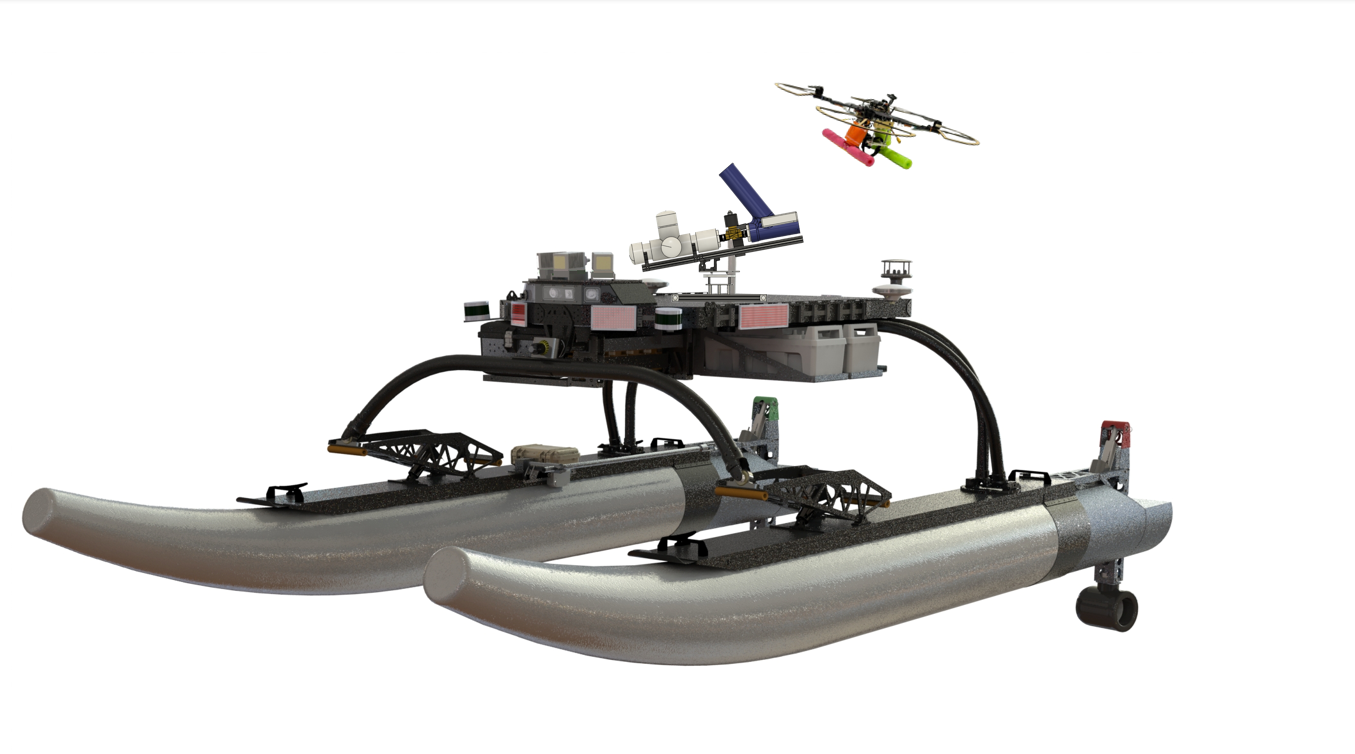
\includegraphics[width=0.8\textwidth]{Images/Minion.png}
\caption{ERAU's \ac{WAMV} Research Vessel Minion as configured for the 2024 Maritime RobotX Challenge.}
\label{fig:minion}
\end{figure}

The sensing configuration used in this research and the 2024 competition is described in Section \ref{perception_geometry}.
% The sensor configuration described in section \ref{perception_geometry} was originally developed by Team Minion for the 2022 and 2024 Maritime RobotX competitions \cite{holland2024, thompson2023}. 
Section~\ref{sensors} presents the technical specifications of Minion's sensor hardware, with particular emphasis on the \ac{LiDAR} and high-definition camera sensors selected for this study.
An overview of the CPU and network infrastructure of the system is provided in section~\ref{sec:Atlas_LAN} as background for the computational requirements of the real-time object detection methods presented in Chapter~\ref{realtime_object_detection}, as well as the challenges relating to the synchronization of sensors in section~\ref{sec:calibration}.
% housed within the forward camera enclosure. Section~\ref{visual_cameras} provides additional discussion regarding visual spectrum sensor selection and characterization. 
Of particular note, the timestamp embedding mechanism described in Section~\ref{time_sync_cam} overcomes network latency issues in the video pipeline to maintain a more precise temporal alignment.
% , essential for rigorous multi-modal sensor fusion analysis.
Finally, section~\ref{sec:sensor_data_dataset} discusses the \ac{ROS} software architecture responsible for recording and processing sensor data.

%%%%%%%%%%%%%%%%%%%%%%%%%%%%%%%%%%%%%%%%%%%%%%%%%%%%%%%%%%%%%%%%%%%%
%%%%%%%%%%%%%%%%%%%%%%%%%%%%%%%%%%%%%%%%%%%%%%%%%%%%%%%%%%%%%%%%%%%%

\section{Perception Geometry} \label{perception_geometry}
\subfile{sections/perception_geometry}

\section{Sensors} \label{sensors}
\subfile{sections/sensors}

\section{Compute Hardware and Network} \label{sec:Atlas_LAN}
\subfile{sections/hardware}

\section{Sensor Calibration} \label{sec:calibration}
\subfile{sections/calibration}

\section{Sensor Data and Dataset} \label{sec:sensor_data_dataset}
\subfile{sections/sensor_data}

\chapter{Real-time Object Detection} \label{realtime_object_detection}


Real-time object detection lies at the core of autonomous perception, enabling vehicles to interpret their surroundings and respond safely to dynamic environments.
Effective detection requires identifying, classifying, and localizing objects rapidly enough to support decision-making and control loops, often under constraints of limited onboard computing and bandwidth.
In this work, these challenges are examined through vision and LiDAR detection pipelines implemented on the Minion sensing platform.

The central focus of this investigation is the development of a late-fusion framework that integrates information from both sensing domains to enhance detection robustness and confidence.
This framework represents the primary contribution of the research and demonstrates how visual and LiDAR detections can be combined at the decision level to exploit the complementary strengths of each sensing modality while mitigating their individual limitations.

To establish a meaningful basis for evaluation, two single-modality detection systems were selected as comparative baselines.
YOLOv8 represents the class of data-driven neural network detectors optimized for vision-based perception, while GB-CACHE represents the class of deterministic, geometry-based algorithms used for LiDAR clustering and segmentation.
These methods were not chosen to exhaust all available detection approaches, but because they are broadly representative of the state of the art within their respective sensing domains.

YOLOv8 was selected for its status as one of the most widely adopted and optimized real-time vision networks, capable of achieving high detection accuracy and efficient inference on GPU-based platforms.
Its inclusion provides a mature and well-understood benchmark for camera-based perception and a reliable reference for evaluating the complementary benefits of late fusion.

GB-CACHE was selected as a deterministic counterpart to YOLO that performs real-time clustering and segmentation without the computational overhead or data dependency of neural network–based LiDAR methods.
Its use of concave-hull extraction provides boundary representations more meaningful for maritime navigation than the simplified 3D bounding boxes produced by models such as PointNet or VoxelNet.
This geometry-driven approach broadens the scope of the comparative study, especially given that the advantages of neural LiDAR methods for real-time deployment remain unproven.

These two approaches represent two distinct strategies for real-time perception, and the late-fusion method developed in this work integrates their complementary strengths to achieve higher confidence detections across a range of operating conditions.
The following sections examine each detection method in sequence.
Section~\ref{yolo} presents the YOLOv8 vision-based detector and its implementation for real-time object recognition.
Section~\ref{gbcache} describes the GB-CACHE algorithm for LiDAR-based clustering and object segmentation.
Finally, Section~\ref{late_fusion} introduces the late-fusion framework developed in this research and evaluates its performance relative to the single-modality detectors through a comparative analysis of detection accuracy, computational efficiency, and real-time operation.

%%%%%%%%%%%%%%%%%%%%%%%%%%%%%%%%%%%%%%%%%%%%%%%%%%%%%%%%%%%%%%%%%%%%
%%%%%%%%%%%%%%%%%%%%%%%%%%%%%%%%%%%%%%%%%%%%%%%%%%%%%%%%%%%%%%%%%%%%

\section{YOLO} \label{yolo}
\subfile{sections/yolo}

\section{GB-CACHE} \label{gbcache}
\subfile{sections/gbcache}

\section{Late Fusion} \label{late_fusion}
\subfile{sections/late_fusion}

\section{Model Performance} \label{performance}
\subfile{sections/performance}

\chapter{Conclusions}


% This chapter will synthesize findings from all three research objectives:
% - Summary of comparative performance results between LiDAR and vision systems
% - Calibration and synchronization framework effectiveness
% - Real-time processing capability validation
% - Implications for ASV perception system design
% - Contribution to maritime autonomous systems knowledge

\section{Research Objective Achievement Summary}
% Placeholder for objective completion summary

\section{Performance Comparison Findings}
% Placeholder for key comparative analysis conclusions

\section{Implications for ASV System Design}
% Placeholder for practical design guidance conclusions


\chapter{Recommendations and Future Work} \label{chap:recommendations}


\section{Recommendations} \label{sec:recommendations}

\section{Future Work} \label{futurework}

This dual-system configuration facilitated the transition of Minion's software during the period of this research.
\ac{ROS} 1 was the operational framework for all research and data collected in this study, however, \ac{ROS} 1 has entered end-of-life for active development.
Consequently, Minion’s software architecture was gradually migrated to \ac{ROS} 2, which introduces substantial improvements in real-time performance, memory management, and inter-process communication.
In contrast to ROS 1’s reliance on a centralized message broker, ROS 2 employs a Data Distribution Service-based communication layer that reduces latency and memory overhead through zero-copy data handling and improved resource allocation.
Maintaining one system on ROS 1 while transitioning the other to ROS 2 allowed incremental software migration without interrupting field operations—laying the groundwork for future runtime performance improvements anticipated in Section~\ref{futurework}.

% This chapter will address:
% - Recommendations for ASV perception system design based on findings
% - Sensor selection guidance for maritime applications
% - Future research directions for maritime sensor fusion
% - Technology transfer opportunities to operational systems

\section{ASV Perception System Design Recommendations}
% Placeholder for design guidance recommendations

\section{Future Research Directions}
% Placeholder for future work recommendations

\section{Technology Transfer Opportunities}
% Placeholder for practical application recommendations




% \printbibliography
% \bibliographystyle{plainnat} - Most recent
\bibliographystyle{IEEEtranN} % natbib-compatible numeric IEEE style
% \bibliography{References}
\bibliography{Dissertation,extra_cite}

\backmatter


\chapter{Image Transform} \label{img_tform}


To obtain the two-dimensional pixel coordinates of the distorted image ($u, v$) in the camera frame $C$ from a three-dimensional coordinate ($X_{L}, Y_L, Z_L$) in the LiDAR frame $L$:

% 3D LiDAR point to distorted image pixel
% \paragraph{Projection from LiDAR to image.}
Let $\mathbf{R}\in \mathbb{R}^{3\times3}$, $\mathbf{t}\in \mathbb{R}^{3\times1}$, $_L\mathbf{P} = [X_L, Y_L, Z_L, 1]^T$,  and $_C\mathbf{P} = \;_{C}^{L}\mathbf{T} \; _L\mathbf{P}$, then:
\begin{equation*}
_C\mathbf{P} = [X_C, Y_C, Z_C, 1]^T \;= \; _{C}^{L}\mathbf{T} \;[X_L, Y_L, Z_L, 1]^T,
% ,\qquad
% _{C}^{L}\mathbf{T} =
% \begin{bmatrix}
% \mathbf{R}_{C}^{L} & \mathbf{t}_{C}^{L} \\
% \mathbf{0}^T & 1
% \end{bmatrix}.
% \label{eq:LiDAR_to_cam_frame}
\end{equation*}

such that:
\begin{equation*}
    _{L}^{C}\mathbf{T} =
    \begin{bmatrix}
        _{L}^{C}\mathbf{R} & _{L}^{C}\mathbf{t} \\
        \mathbf{0}^\mathrm{T} & 1
    \end{bmatrix},
\end{equation*}

We obtain the pixel coordinates ($x_n, y_n$) in the undistorted image frame by pinhole projection:
\begin{equation*}
x_n = \frac{X_C}{Z_C}, \qquad
y_n = \frac{Y_C}{Z_C}, \qquad
r^2 = x_n^2 + y_n^2 .
\label{eq:normalized_coords}
\end{equation*}

Apply the radial distortion model:
\begin{align*}
r^2 & = x_n^2 + y_n^2 .\\
x' & = x_n\!\left(1 + k_1 r^2 + k_2 r^4 + k_3 r^6\right), \\
y' & = y_n\!\left(1 + k_1 r^2 + k_2 r^4 + k_3 r^6\right).
\label{eq:radial_distortion_apply}
\end{align*}

Map ($x', y'$) to distorted pixel coordinates ($u,v$) using the intrinsic matrix $\mathbf{K}$:
\begin{equation}
\begin{bmatrix} u \\ v \\ 1 \end{bmatrix}
=
\begin{bmatrix}
f_x & s & c_x \\
0   & f_y & c_y \\
0   & 0   & 1
\end{bmatrix}
\begin{bmatrix} x' \\ y' \\ 1 \end{bmatrix},
\qquad
% \mathbf{K} =
% \begin{bmatrix}
% f_x & s & c_x \\
% 0   & f_y & c_y \\
% 0   & 0   & 1
% \end{bmatrix},
% \quad
\Rightarrow\ 
\begin{cases}
u = f_x x' + s y' + c_x,\\
v = f_y y' + c_y.
\end{cases}
\label{eq:intrinsics_to_pixels}
\end{equation}

% \chapter{test 2}

% \begin{figure}[htbp]
%        \centering
%        % TikZ Flowchart for GStreamer HDR Pipeline
% Drop-in code for Overleaf
% Requires: \usepackage{tikz}
%          \usetikzlibrary{shapes.geometric, arrows}

\tikzstyle{process} = [rectangle, minimum width=3cm, minimum height=1cm, text centered, draw=black, fill=white, text width=3cm]
\tikzstyle{timestamp} = [rectangle, minimum width=3cm, minimum height=1cm, text centered, draw=red, line width=1.5pt, fill=white, text width=3cm]
\tikzstyle{queue} = [rectangle, minimum width=2.5cm, minimum height=0.8cm, text centered, draw=blue, line width=1.2pt, fill=white, text width=2.5cm]
\tikzstyle{output} = [rectangle, minimum width=2.5cm, minimum height=1cm, text centered, draw=green!60!black, line width=1.2pt, fill=white, text width=2.5cm, rounded corners]
\tikzstyle{decision} = [diamond, minimum width=2cm, minimum height=1cm, text centered, draw=black, fill=white, aspect=2]
\tikzstyle{arrow} = [thick,->,>=stealth]

\begin{tikzpicture}[node distance=2cm]

% Source
\node (source) [process] {\textbf{v4l2src / videotestsrc} \\ YUY2, 2880x1860@60fps \\ do-timestamp=TRUE};

% Timestamp Probe 1
\node (ts1) [timestamp, below of=source] {\textbf{TIMESTAMP PROBE \#1} \\ timestamp\_probe\_cb \\ Adds CustomTimestampMeta \\ gettimeofday() $\rightarrow$ ms};

% Tee
\node (tee) [decision, below of=ts1, yshift=-0.5cm] {\textbf{TEE (Splits 3x)}};

% Stream Branch (left)
\node (qs) [queue, below of=tee, xshift=-8cm, yshift=-1.5cm] {\textbf{queue\_stream} \\ {[BUFFER QUEUE]}};
\node (vr) [process, below of=qs] {\textbf{videorate} \\ 60fps $\rightarrow$ 5fps};
\node (nvc1) [process, below of=vr] {\textbf{nvvidconv} \\ YUY2 $\rightarrow$ I420 \\ NVMM memory};
\node (h264e) [process, below of=nvc1] {\textbf{nvv4l2h264enc} \\ H264 encode \\ bitrate=calc \\ insert-sps-pps=true};
\node (sei) [timestamp, below of=h264e] {\textbf{TIMESTAMP PROBE \#2} \\ sei\_insert\_probe\_cb \\ Reads CustomTimestampMeta \\ Inserts SEI NAL unit};
\node (h264p) [process, below of=sei] {\textbf{h264parse} \\ Parse H264 stream};
\node (rtp) [process, below of=h264p] {\textbf{rtph264pay} \\ RTP payload \\ config-interval=1 \\ mtu=1400};
\node (udp) [output, below of=rtp] {\textbf{udpsink} \\ host=201.7.90.18 \\ port=5603 \\ sync=false};

% Record Branch (middle)
\node (qr) [queue, below of=tee, yshift=-1.5cm] {\textbf{queue\_record} \\ {[BUFFER QUEUE]}};
\node (nvc2) [process, below of=qr] {\textbf{nvvidconv} \\ YUY2 $\rightarrow$ I420 \\ NVMM memory};
\node (h265e) [process, below of=nvc2] {\textbf{nvv4l2h265enc} \\ H265 encode \\ bitrate=80Mbps \\ iframeinterval=1};
\node (h265p) [process, below of=h265e] {\textbf{h265parse} \\ Parse H265 \\ byte-stream};
\node (split) [output, below of=h265p, yshift=-1cm] {\textbf{splitmuxsink} \\ muxer=qtmux \\ Split @120s \\ /mnt/logs/hdr-0/ \\ hdr-0-\{time\}-\{n\}.mp4};

% CSV Branch (right)
\node (qc) [queue, below of=tee, xshift=8cm, yshift=-1.5cm] {\textbf{queue} \\ {[BUFFER QUEUE]}};
\node (id) [process, below of=qc] {\textbf{identity} \\ csv\_identity \\ signal-handoffs=true};
\node (csv) [timestamp, below of=id] {\textbf{TIMESTAMP LOGGER} \\ csv\_handoff\_handler \\ Reads CustomTimestampMeta \\ Logs: frame\#,timestamp};
\node (csvf) [output, below of=csv, xshift=-2.5cm, yshift=-0.5cm] {\textbf{CSV Files} \\ /mnt/logs/hdr-0/ \\ hdr-0-\{time\}-\{n\}.csv \\ Split @120s};
\node (fake) [output, below of=csv, xshift=2.5cm, yshift=-0.5cm] {\textbf{fakesink} \\ discard};

% Arrows
\draw [arrow] (source) -- (ts1);
\draw [arrow] (ts1) -- node[anchor=east, xshift=-0.3cm] {[BUFFER + Metadata]} (tee);

% Stream branch arrows
\draw [arrow] (tee) -| node[anchor=south, yshift=0.3cm, xshift=-4cm] {Stream Branch} (qs);
\draw [arrow] (qs) -- (vr);
\draw [arrow] (vr) -- (nvc1);
\draw [arrow] (nvc1) -- (h264e);
\draw [arrow] (h264e) -- (sei);
\draw [arrow] (sei) -- node[anchor=east, xshift=-0.3cm] {[H264 + SEI NAL]} (h264p);
\draw [arrow] (h264p) -- (rtp);
\draw [arrow] (rtp) -- node[anchor=east, xshift=-0.3cm] {[RTP Packets]} (udp);

% Record branch arrows
\draw [arrow] (tee) -- node[anchor=east, xshift=-0.3cm] {Record Branch} (qr);
\draw [arrow] (qr) -- (nvc2);
\draw [arrow] (nvc2) -- (h265e);
\draw [arrow] (h265e) -- (h265p);
\draw [arrow] (h265p) -- (split);

% CSV branch arrows
\draw [arrow] (tee) -| node[anchor=south, yshift=0.3cm, xshift=4cm] {CSV Branch} (qc);
\draw [arrow] (qc) -- (id);
\draw [arrow] (id) -- (csv);
\draw [arrow] (csv) -- (csvf);
\draw [arrow] (csv) -- (fake);

\end{tikzpicture}

%        \caption{GStreamer pipeline architecture for HDR camera streaming, 
%                 recording, and timestamp logging.}
%        \label{fig:hdr_pipeline}
%    \end{figure}


\end{document}


% \bibliographystyle{plainnat} - Most recent
\bibliographystyle{IEEEtranN} % natbib-compatible numeric IEEE style
% \bibliography{References}
\bibliography{Dissertation,extra_cite}

\backmatter

\chapter{Image Transform} \label{img_tform}

To obtain the two-dimensional pixel coordinates of the distorted image ($u, v$) in the camera frame $C$ from a three-dimensional coordinate ($X_{L}, Y_L, Z_L$) in the LiDAR frame $L$:

% 3D LiDAR point to distorted image pixel
% \paragraph{Projection from LiDAR to image.}
Let $\mathbf{R}\in \mathbb{R}^{3\times3}$, $\mathbf{t}\in \mathbb{R}^{3\times1}$, $_L\mathbf{P} = [X_L, Y_L, Z_L, 1]^T$,  and $_C\mathbf{P} = \;_{C}^{L}\mathbf{T} \; _L\mathbf{P}$, then:
\begin{equation*}
_C\mathbf{P} = [X_C, Y_C, Z_C, 1]^T \;= \; _{C}^{L}\mathbf{T} \;[X_L, Y_L, Z_L, 1]^T,
% ,\qquad
% _{C}^{L}\mathbf{T} =
% \begin{bmatrix}
% \mathbf{R}_{C}^{L} & \mathbf{t}_{C}^{L} \\
% \mathbf{0}^T & 1
% \end{bmatrix}.
% \label{eq:LiDAR_to_cam_frame}
\end{equation*}

such that:
\begin{equation*}
    _{L}^{C}\mathbf{T} =
    \begin{bmatrix}
        _{L}^{C}\mathbf{R} & _{L}^{C}\mathbf{t} \\
        \mathbf{0}^\mathrm{T} & 1
    \end{bmatrix},
\end{equation*}

We obtain the pixel coordinates ($x_n, y_n$) in the undistorted image frame by pinhole projection:
\begin{equation*}
x_n = \frac{X_C}{Z_C}, \qquad
y_n = \frac{Y_C}{Z_C}, \qquad
r^2 = x_n^2 + y_n^2 .
\label{eq:normalized_coords}
\end{equation*}

Apply the radial distortion model:
\begin{align*}
r^2 & = x_n^2 + y_n^2 .\\
x' & = x_n\!\left(1 + k_1 r^2 + k_2 r^4 + k_3 r^6\right), \\
y' & = y_n\!\left(1 + k_1 r^2 + k_2 r^4 + k_3 r^6\right).
\label{eq:radial_distortion_apply}
\end{align*}

Map ($x', y'$) to distorted pixel coordinates ($u,v$) using the intrinsic matrix $\mathbf{K}$:
\begin{equation}
\begin{bmatrix} u \\ v \\ 1 \end{bmatrix}
=
\begin{bmatrix}
f_x & s & c_x \\
0   & f_y & c_y \\
0   & 0   & 1
\end{bmatrix}
\begin{bmatrix} x' \\ y' \\ 1 \end{bmatrix},
\qquad
% \mathbf{K} =
% \begin{bmatrix}
% f_x & s & c_x \\
% 0   & f_y & c_y \\
% 0   & 0   & 1
% \end{bmatrix},
% \quad
\Rightarrow\ 
\begin{cases}
u = f_x x' + s y' + c_x,\\
v = f_y y' + c_y.
\end{cases}
\label{eq:intrinsics_to_pixels}
\end{equation}

% \chapter{test 2}

% \begin{figure}[htbp]
%        \centering
%        % TikZ Flowchart for GStreamer HDR Pipeline
% Drop-in code for Overleaf
% Requires: \usepackage{tikz}
%          \usetikzlibrary{shapes.geometric, arrows}

\tikzstyle{process} = [rectangle, minimum width=3cm, minimum height=1cm, text centered, draw=black, fill=white, text width=3cm]
\tikzstyle{timestamp} = [rectangle, minimum width=3cm, minimum height=1cm, text centered, draw=red, line width=1.5pt, fill=white, text width=3cm]
\tikzstyle{queue} = [rectangle, minimum width=2.5cm, minimum height=0.8cm, text centered, draw=blue, line width=1.2pt, fill=white, text width=2.5cm]
\tikzstyle{output} = [rectangle, minimum width=2.5cm, minimum height=1cm, text centered, draw=green!60!black, line width=1.2pt, fill=white, text width=2.5cm, rounded corners]
\tikzstyle{decision} = [diamond, minimum width=2cm, minimum height=1cm, text centered, draw=black, fill=white, aspect=2]
\tikzstyle{arrow} = [thick,->,>=stealth]

\begin{tikzpicture}[node distance=2cm]

% Source
\node (source) [process] {\textbf{v4l2src / videotestsrc} \\ YUY2, 2880x1860@60fps \\ do-timestamp=TRUE};

% Timestamp Probe 1
\node (ts1) [timestamp, below of=source] {\textbf{TIMESTAMP PROBE \#1} \\ timestamp\_probe\_cb \\ Adds CustomTimestampMeta \\ gettimeofday() $\rightarrow$ ms};

% Tee
\node (tee) [decision, below of=ts1, yshift=-0.5cm] {\textbf{TEE (Splits 3x)}};

% Stream Branch (left)
\node (qs) [queue, below of=tee, xshift=-8cm, yshift=-1.5cm] {\textbf{queue\_stream} \\ {[BUFFER QUEUE]}};
\node (vr) [process, below of=qs] {\textbf{videorate} \\ 60fps $\rightarrow$ 5fps};
\node (nvc1) [process, below of=vr] {\textbf{nvvidconv} \\ YUY2 $\rightarrow$ I420 \\ NVMM memory};
\node (h264e) [process, below of=nvc1] {\textbf{nvv4l2h264enc} \\ H264 encode \\ bitrate=calc \\ insert-sps-pps=true};
\node (sei) [timestamp, below of=h264e] {\textbf{TIMESTAMP PROBE \#2} \\ sei\_insert\_probe\_cb \\ Reads CustomTimestampMeta \\ Inserts SEI NAL unit};
\node (h264p) [process, below of=sei] {\textbf{h264parse} \\ Parse H264 stream};
\node (rtp) [process, below of=h264p] {\textbf{rtph264pay} \\ RTP payload \\ config-interval=1 \\ mtu=1400};
\node (udp) [output, below of=rtp] {\textbf{udpsink} \\ host=201.7.90.18 \\ port=5603 \\ sync=false};

% Record Branch (middle)
\node (qr) [queue, below of=tee, yshift=-1.5cm] {\textbf{queue\_record} \\ {[BUFFER QUEUE]}};
\node (nvc2) [process, below of=qr] {\textbf{nvvidconv} \\ YUY2 $\rightarrow$ I420 \\ NVMM memory};
\node (h265e) [process, below of=nvc2] {\textbf{nvv4l2h265enc} \\ H265 encode \\ bitrate=80Mbps \\ iframeinterval=1};
\node (h265p) [process, below of=h265e] {\textbf{h265parse} \\ Parse H265 \\ byte-stream};
\node (split) [output, below of=h265p, yshift=-1cm] {\textbf{splitmuxsink} \\ muxer=qtmux \\ Split @120s \\ /mnt/logs/hdr-0/ \\ hdr-0-\{time\}-\{n\}.mp4};

% CSV Branch (right)
\node (qc) [queue, below of=tee, xshift=8cm, yshift=-1.5cm] {\textbf{queue} \\ {[BUFFER QUEUE]}};
\node (id) [process, below of=qc] {\textbf{identity} \\ csv\_identity \\ signal-handoffs=true};
\node (csv) [timestamp, below of=id] {\textbf{TIMESTAMP LOGGER} \\ csv\_handoff\_handler \\ Reads CustomTimestampMeta \\ Logs: frame\#,timestamp};
\node (csvf) [output, below of=csv, xshift=-2.5cm, yshift=-0.5cm] {\textbf{CSV Files} \\ /mnt/logs/hdr-0/ \\ hdr-0-\{time\}-\{n\}.csv \\ Split @120s};
\node (fake) [output, below of=csv, xshift=2.5cm, yshift=-0.5cm] {\textbf{fakesink} \\ discard};

% Arrows
\draw [arrow] (source) -- (ts1);
\draw [arrow] (ts1) -- node[anchor=east, xshift=-0.3cm] {[BUFFER + Metadata]} (tee);

% Stream branch arrows
\draw [arrow] (tee) -| node[anchor=south, yshift=0.3cm, xshift=-4cm] {Stream Branch} (qs);
\draw [arrow] (qs) -- (vr);
\draw [arrow] (vr) -- (nvc1);
\draw [arrow] (nvc1) -- (h264e);
\draw [arrow] (h264e) -- (sei);
\draw [arrow] (sei) -- node[anchor=east, xshift=-0.3cm] {[H264 + SEI NAL]} (h264p);
\draw [arrow] (h264p) -- (rtp);
\draw [arrow] (rtp) -- node[anchor=east, xshift=-0.3cm] {[RTP Packets]} (udp);

% Record branch arrows
\draw [arrow] (tee) -- node[anchor=east, xshift=-0.3cm] {Record Branch} (qr);
\draw [arrow] (qr) -- (nvc2);
\draw [arrow] (nvc2) -- (h265e);
\draw [arrow] (h265e) -- (h265p);
\draw [arrow] (h265p) -- (split);

% CSV branch arrows
\draw [arrow] (tee) -| node[anchor=south, yshift=0.3cm, xshift=4cm] {CSV Branch} (qc);
\draw [arrow] (qc) -- (id);
\draw [arrow] (id) -- (csv);
\draw [arrow] (csv) -- (csvf);
\draw [arrow] (csv) -- (fake);

\end{tikzpicture}

%        \caption{GStreamer pipeline architecture for HDR camera streaming, 
%                 recording, and timestamp logging.}
%        \label{fig:hdr_pipeline}
%    \end{figure}


\end{document}

